\documentclass[11pt]{article}
\usepackage{amsmath,amssymb,amsthm}
\usepackage{tikz}
\usetikzlibrary{positioning}
\usepackage{booktabs}
\usepackage{array}
\usepackage{geometry}
\geometry{margin=1in}
\setlength{\parindent}{0pt}
\setlength{\parskip}{6pt}

\newtheorem*{claim}{Claim}

\begin{document}

\begin{center}
  {\large\bfseries COSC 4P04 --- Assignment 4}
\end{center}

\section*{Question 1: Stable Matching}

\subsection*{(a) Gale-Shapley (hospital-proposing)}

Doctor preferences: X: B$>$A$>$C \quad Y: A$>$B$>$C \quad Z: A$>$B$>$C\\
Hospital preferences: A: X$>$Y$>$Z \quad B: Y$>$X$>$Z \quad C: X$>$Y$>$Z

\textbf{Round 1.}
A proposes to X, B proposes to Y, C proposes to X.\\
X receives \{A,C\}: X prefers A over C $\Rightarrow$ X holds A, rejects C.\\
Y receives \{B\}: Y holds B.\\
Z receives nothing.

\textbf{Round 2.}
C proposes to Y (next on C's list).\\
Y receives \{B,C\}: Y prefers B over C $\Rightarrow$ Y holds B, rejects C.\\
Z still receives nothing.

\textbf{Round 3.}
C proposes to Z (last on C's list).\\
Z receives \{C\}: Z holds C.

\textbf{Result:} $\{X\text{--}A,\; Y\text{--}B,\; Z\text{--}C\}$.

\subsection*{(b) All stable matchings}

We test every possible perfect matching.

\textbf{Matching 1:} $\{X\text{--}A, Y\text{--}B, Z\text{--}C\}$ (GS result).\\
Check all pairs not in the matching:
$(X,B)$: X prefers B$>$A but B prefers Y$>$X, so B does not want to leave Y. Not blocking.\\
$(Y,A)$: Y prefers A$>$B but A prefers X$>$Y, so A does not want to leave X. Not blocking.\\
$(Z,A),(Z,B)$: A prefers X$>$Y$>$Z; B prefers Y$>$X$>$Z --- neither hospital prefers Z over its current match. Not blocking.\\
\textbf{Stable.}

\textbf{Matching 2:} $\{X\text{--}B, Y\text{--}A, Z\text{--}C\}$.\\
$(X,A)$: X prefers B$>$A, so X does not want A. Not blocking.\\
$(Y,B)$: Y prefers A$>$B, so Y does not want B. Not blocking.\\
$(Z,A)$: Z prefers A; A prefers X$>$Y$>$Z but A is already with Y, and A prefers Y$>$Z. Not blocking.\\
$(Z,B)$: B prefers Y$>$X$>$Z; B is with X and prefers X$>$Z. Not blocking.\\
\textbf{Stable.}

\textbf{Other matchings} all contain a blocking pair:
$\{X\text{--}A, Y\text{--}C, Z\text{--}B\}$: $(Y,B)$ is blocking (Y prefers B$>$C; B is with Z and prefers Y$>$X$>$Z).\\
$\{X\text{--}C, Y\text{--}A, Z\text{--}B\}$: $(X,B)$ is blocking (X prefers B$>$C; B is with Z and prefers X$>$Z).\\
$\{X\text{--}B, Y\text{--}C, Z\text{--}A\}$: $(Y,A)$ is blocking (Y prefers A$>$C; A is with Z and prefers Y$>$Z).\\
$\{X\text{--}C, Y\text{--}B, Z\text{--}A\}$: $(X,A)$ is blocking (X prefers A$>$C; A is with Z and prefers X$>$Z).

\textbf{There are exactly 2 stable matchings.}

\subsection*{(c) Hospitals are matched with best(A) --- proof}

\begin{claim}
In hospital-proposing Gale-Shapley every hospital $H$ is matched with $\mathrm{best}(H)$, its highest-ranked feasible partner.
\end{claim}
\begin{proof}
Suppose for contradiction that some hospital $H$ is not matched with $\mathrm{best}(H)$.  Let $H$ be the \emph{first} hospital to be rejected by a feasible partner during GS execution, and let $d^*$ be that feasible partner ($H$ proposed to $d^*$ and $d^*$ rejected $H$ in favour of some hospital $H'$).

Because $d^*$ is feasible for $H$ there exists a stable matching $M$ where $H$ is matched with $d^*$.  In $M$, let $H'$ be matched with doctor $d'$.

We show $(d^*, H')$ is a blocking pair in $M$:
\begin{enumerate}
  \item $d^*$ prefers $H'$ over $H$: $d^*$ rejected $H$ in favour of $H'$ during GS, so $d^* \succ_{d^*} H'$ over $H$.
  \item $H'$ prefers $d^*$ over $d'$: Since $H$ was the \emph{first} hospital rejected by a feasible partner, $H'$ had not yet been rejected by any feasible partner when $d^*$ accepted $H'$.  In GS, hospitals propose in decreasing preference order, so $H'$ proposed to $d^*$ (and $d^*$ accepted) before $H'$ could have proposed to $d'$.  Hence $d^*$ ranks higher on $H'$'s list than $d'$, i.e.\ $H' \succ_{H'} d^*$ over $d'$.
\end{enumerate}

Thus $(d^*,H')$ blocks $M$, contradicting $M$ being stable.  Therefore every hospital is matched with $\mathrm{best}(H)$.
\end{proof}

In our example, $\mathrm{best}(A)=X$ (A's top choice, feasible in Matching 1).  GS gives $A$--$X$.  Similarly $\mathrm{best}(B)=Y$ and GS gives $B$--$Y$. $\checkmark$

\subsection*{(d) Doctors are matched with worst($\alpha$) --- proof}

\begin{claim}
In hospital-proposing Gale-Shapley every doctor $\alpha$ is matched with $\mathrm{worst}(\alpha)$, their lowest-ranked feasible hospital.
\end{claim}
\begin{proof}
Let $\alpha$ be matched with $H$ in GS.  Take any stable matching $M$ where $\alpha$ is matched with $H'$.  We show $\alpha$ prefers $H$ over $H'$ (i.e.\ $H$ is at least as bad for $\alpha$ as $H'$, so $H$ is the worst).

By (c), $H$'s GS partner is $\mathrm{best}(H)$.  Since $\alpha$ is $H$'s GS partner, $\alpha = \mathrm{best}(H)$, meaning $H$ prefers $\alpha$ over any doctor it could be matched with in a stable matching, including $d'$ (H's partner in $M$).

Suppose for contradiction that $\alpha$ prefers $H'$ over $H$.  In $M$: $\alpha$ is with $H'$ and H is with some $d'$.  Then:
(i) $\alpha$ prefers $H'$ (by assumption), and
(ii) $H$ prefers $\alpha$ over $d'$ (since $\alpha = \mathrm{best}(H)$).

So $(\alpha, H)$ is a blocking pair in $M$, contradicting $M$ being stable.  Therefore $\alpha$ does not prefer any stable-matching partner over $H$, i.e.\ $H = \mathrm{worst}(\alpha)$.
\end{proof}

In our example, $\mathrm{worst}(X) = A$ (only stable matching giving X the worst is X--A) and $\mathrm{worst}(Y) = B$; both verified from the two stable matchings.

\subsection*{(e) Doctor-proposing Gale-Shapley}

\textbf{Round 1.}
X proposes to B, Y proposes to A, Z proposes to A.\\
B receives \{X\}: B holds X.\\
A receives \{Y,Z\}: A prefers Y$>$Z $\Rightarrow$ A holds Y, rejects Z.

\textbf{Round 2.}
Z proposes to B (next on Z's list).\\
B receives \{X,Z\}: B prefers X$>$Z $\Rightarrow$ B holds X, rejects Z.

\textbf{Round 3.}
Z proposes to C.  C holds Z.

\textbf{Result:} $\{X\text{--}B,\; Y\text{--}A,\; Z\text{--}C\}$.

\textbf{Comparison:}
\begin{center}
\begin{tabular}{lcc}
\toprule
 & Hospital-proposing & Doctor-proposing \\
\midrule
X gets & A (2nd choice) & B (1st choice) \\
Y gets & B (2nd choice) & A (1st choice) \\
Z gets & C (3rd choice) & C (3rd choice) \\
A gets & X (1st choice) & Y (2nd choice) \\
B gets & Y (1st choice) & X (2nd choice) \\
\bottomrule
\end{tabular}
\end{center}

Yes, doctor-proposing GS is advantageous for doctors (X and Y both receive their first choice) and less favourable for hospitals.  This illustrates that GS is optimal for the proposing side.

\newpage
\section*{Question 2: BFS and DFS}

The graph $G$ used throughout (Figure 1):

\begin{center}
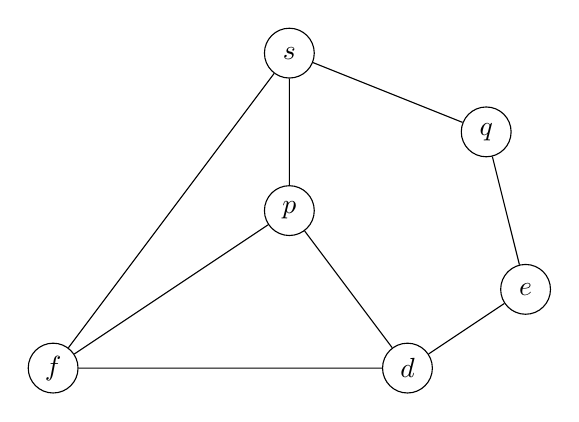
\begin{tikzpicture}[every node/.style={circle,draw,inner sep=2pt,minimum size=18pt},
                    every edge/.style={draw}]
  \node (s) at (3,4)   {$s$};
  \node (q) at (5.5,3) {$q$};
  \node (p) at (3,2)   {$p$};
  \node (e) at (6,1)   {$e$};
  \node (f) at (0,0)   {$f$};
  \node (d) at (4.5,0) {$d$};
  \draw (s)--(q) (s)--(p) (s)--(f) (p)--(d) (p)--(f) (q)--(e) (d)--(e) (d)--(f);
\end{tikzpicture}
\end{center}

Adjacency lists (alphabetical order):
$d$: $e,f,p$ \quad $e$: $d,q$ \quad $f$: $d,p,s$ \quad $p$: $d,f,s$ \quad $q$: $e,s$ \quad $s$: $f,p,q$

\subsection*{(a) Whatever-First Search from $s$}

Using the WFS algorithm from~[2] (mark neighbours on insertion):

\begin{center}
\begin{tabular}{cll}
\toprule
Step & Node visited & Bag after step \\
\midrule
1 & $s$ & $\{f,p,q\}$ \\
2 & $f$ & $\{p,q,d\}$ \quad ($d$ newly marked) \\
3 & $p$ & $\{q,d\}$ \quad (all $p$-neighbours already marked) \\
4 & $q$ & $\{d,e\}$ \quad ($e$ newly marked) \\
5 & $d$ & $\{e\}$ \quad (all $d$-neighbours already marked) \\
6 & $e$ & $\{\}$ \quad (all $e$-neighbours already marked) \\
\bottomrule
\end{tabular}
\end{center}

Visit order: $s, f, p, q, d, e$.

\subsection*{(b) BFS using a \textquotedblleft stack\textquotedblright}

As required by the question, we run WFS with a \textbf{stack} (LIFO) bag. This in fact produces \textbf{depth-first} traversal, demonstrating that the data structure determines the traversal order.

\begin{center}
\begin{tabular}{clll}
\toprule
Step & Popped & Stack after (top on right) & Newly marked \\
\midrule
1 & $s$ & $[f, p, q]$ & $f, p, q$ \\
2 & $q$ & $[f, p, e]$ & $e$ \\
3 & $e$ & $[f, p, d]$ & $d$ \\
4 & $d$ & $[f, p]$   & (none) \\
5 & $p$ & $[f]$       & (none) \\
6 & $f$ & $[\;]$      & (none) \\
\bottomrule
\end{tabular}
\end{center}

Visit order: $s, q, e, d, p, f$.

\textbf{Observation:} using a stack produces a \emph{DFS} traversal, not BFS.  The data structure choice determines the traversal type.

\subsection*{(c) Iterative DFS using a \textquotedblleft queue\textquotedblright}

As required by the question, we run WFS with a \textbf{queue} (FIFO) bag. This in fact produces \textbf{breadth-first} traversal, further confirming that the bag type governs the traversal order.

\begin{center}
\begin{tabular}{clll}
\toprule
Step & Dequeued & Queue after (front on left) & Newly marked \\
\midrule
1 & $s$ & $[f, p, q]$ & $f, p, q$ \\
2 & $f$ & $[p, q, d]$ & $d$ \\
3 & $p$ & $[q, d]$    & (none) \\
4 & $q$ & $[d, e]$    & $e$ \\
5 & $d$ & $[e]$       & (none) \\
6 & $e$ & $[\;]$      & (none) \\
\bottomrule
\end{tabular}
\end{center}

Visit order: $s, f, p, q, d, e$.

\textbf{Observation:} using a queue produces a \emph{BFS} traversal.

\newpage
\section*{Question 3: Minimum Spanning Trees}

The weighted graph $G_{\mathrm{mst}}$:

\begin{center}
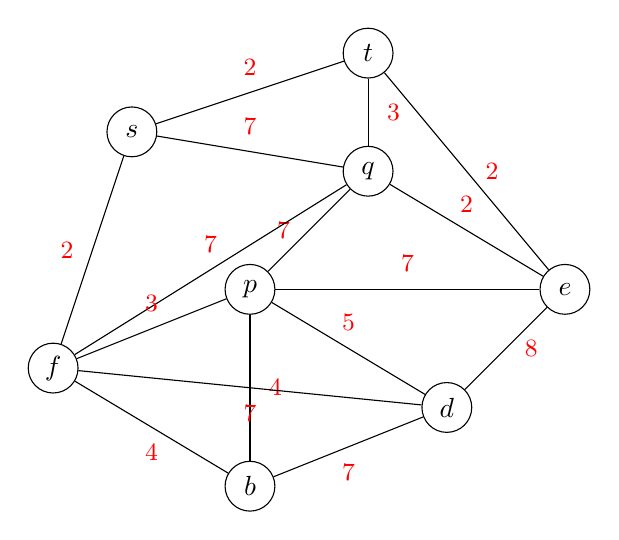
\begin{tikzpicture}[every node/.style={circle,draw,inner sep=2pt,minimum size=18pt},
                    every edge/.style={draw},
                    lbl/.style={draw=none,fill=none,font=\small,red}]
  \node (t) at (5,6)   {$t$};
  \node (s) at (2,5)   {$s$};
  \node (q) at (5,4.5) {$q$};
  \node (e) at (7.5,3) {$e$};
  \node (p) at (3.5,3) {$p$};
  \node (f) at (1,2)   {$f$};
  \node (d) at (6,1.5) {$d$};
  \node (b) at (3.5,.5){$b$};
  \draw (s)--(t) node[lbl,midway,above]{2};
  \draw (s)--(q) node[lbl,midway,above]{7};
  \draw (s)--(f) node[lbl,midway,left]{2};
  \draw (t)--(q) node[lbl,midway,right]{3};
  \draw (t)--(e) node[lbl,midway,right]{2};
  \draw (q)--(e) node[lbl,midway,above]{2};
  \draw (q)--(p) node[lbl,midway,left]{7};
  \draw (q)--(f) node[lbl,midway,above]{7};
  \draw (p)--(f) node[lbl,midway,above]{3};
  \draw (p)--(e) node[lbl,midway,above]{7};
  \draw (p)--(d) node[lbl,midway,above]{5};
  \draw (p)--(b) node[lbl,midway,right]{4};
  \draw (f)--(b) node[lbl,midway,below]{4};
  \draw (b)--(d) node[lbl,midway,below]{7};
  \draw (d)--(e) node[lbl,midway,right]{8};
  \draw (f)--(d) node[lbl,midway,below]{7};
\end{tikzpicture}
\end{center}

\subsection*{(a) Kruskal's algorithm --- $T_k$}

Sort edges by weight (ties broken alphabetically by endpoint names):
\[
(e,t):2,\;(f,s):2,\;(q,e):2,\;(s,t):2,\;(f,p):3,\;(q,t):3,\;(b,f):4,\;(b,p):4,\;(d,p):5,\;\ldots
\]

\begin{center}
\begin{tabular}{llll}
\toprule
Edge & Weight & Action & Components \\
\midrule
$e$--$t$ & 2 & Add & $\{e,t\},\{s\},\{q\},\{p\},\{f\},\{d\},\{b\}$ \\
$f$--$s$ & 2 & Add & $\{e,t\},\{f,s\},\{q\},\{p\},\{d\},\{b\}$ \\
$q$--$e$ & 2 & Add & $\{e,q,t\},\{f,s\},\{p\},\{d\},\{b\}$ \\
$s$--$t$ & 2 & Add & $\{e,f,q,s,t\},\{p\},\{d\},\{b\}$ \\
$f$--$p$ & 3 & Add & $\{e,f,p,q,s,t\},\{d\},\{b\}$ \\
$q$--$t$ & 3 & Skip & cycle \\
$b$--$f$ & 4 & Add & $\{b,e,f,p,q,s,t\},\{d\}$ \\
$b$--$p$ & 4 & Skip & cycle \\
$d$--$p$ & 5 & Add & $\{b,d,e,f,p,q,s,t\}$ \quad \textbf{done} \\
\bottomrule
\end{tabular}
\end{center}

$T_k = \{e\text{-}t,\; f\text{-}s,\; q\text{-}e,\; s\text{-}t,\; f\text{-}p,\; b\text{-}f,\; d\text{-}p\}$, \quad total weight $= 2+2+2+2+3+4+5 = \mathbf{20}$.

\subsection*{(b) Prim's algorithm --- $T_p$}

Starting from $s$, maintaining a min-priority queue on key values:

\begin{center}
\begin{tabular}{lll}
\toprule
Extracted node (key) & Edge added & Newly updated keys \\
\midrule
$s$ (0) & --- & $t{\to}2,\; f{\to}2,\; q{\to}7$ \\
$f$ (2) & $s$--$f$ & $b{\to}4,\; d{\to}7,\; p{\to}3$ \\
$t$ (2) & $s$--$t$ & $e{\to}2,\; q{\to}\min(7,3)=3$ \\
$e$ (2) & $t$--$e$ & $q{\to}\min(3,2)=2$ \\
$q$ (2) & $e$--$q$ & (no improvement) \\
$p$ (3) & $f$--$p$ & $d{\to}\min(7,5)=5$ \\
$b$ (4) & $f$--$b$ & (no improvement) \\
$d$ (5) & $p$--$d$ & \textbf{done} \\
\bottomrule
\end{tabular}
\end{center}

$T_p = \{s\text{-}f,\; s\text{-}t,\; t\text{-}e,\; e\text{-}q,\; f\text{-}p,\; f\text{-}b,\; p\text{-}d\}$, \quad total weight $= 2+2+2+2+3+4+5 = \mathbf{20}$.

\subsection*{(c) Are $T_k$ and $T_p$ the same?}

Yes.  Both trees contain exactly the same seven edges:
\[
\{s\text{-}t,\; s\text{-}f,\; t\text{-}e,\; q\text{-}e,\; p\text{-}f,\; f\text{-}b,\; p\text{-}d\}
\]
with total weight 20.  The MST is unique in this graph because the only potential ambiguity (weight-4 tie between $b$-$f$ and $b$-$p$) resolves to $b$-$f$ under any consistent tie-breaking: $f$ is added to the growing tree before $p$ in Prim's, so $f$ sets $\mathrm{pred}[b]$; and $f < p$ alphabetically in Kruskal's.  Hence $T_k = T_p$.

\newpage
\section*{Question 4: Bonus}

\subsection*{(a) A graph with exactly one MST}

Take $G_{\mathrm{unique}}$ with three vertices $a,b,c$ and edges $a$--$b$ (weight~1), $b$--$c$ (weight~2), $a$--$c$ (weight~4).  The unique MST is $\{a\text{-}b,\; b\text{-}c\}$ with weight~3 (adding $a$--$c$ would create a cycle at a higher cost).

\begin{center}
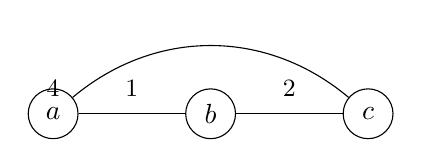
\begin{tikzpicture}[every node/.style={circle,draw,inner sep=2pt,minimum size=18pt},
                    lbl/.style={draw=none,fill=none,font=\small}]
  \node (a) at (0,0) {$a$};
  \node (b) at (2,0) {$b$};
  \node (c) at (4,0) {$c$};
  \draw (a)--(b) node[lbl,above,midway]{1};
  \draw (b)--(c) node[lbl,above,midway]{2};
  \draw (a) to[bend left=40] (c) node[lbl,above,midway]{4};
\end{tikzpicture}
\end{center}

\subsection*{(b) Unique edge weights imply a unique MST}

\begin{claim}
If all edge weights in a connected graph $G$ are distinct, then $G$ has a unique MST.
\end{claim}
\begin{proof}
Suppose $T_1$ and $T_2$ are both MSTs of $G$ with $T_1\neq T_2$.  Let $e$ be the minimum-weight edge in the symmetric difference $T_1\mathbin{\triangle}T_2$; without loss of generality $e\in T_1\setminus T_2$.

Adding $e$ to $T_2$ creates a unique cycle $C$ in $T_2$.  Because $T_1$ is a spanning tree, $C$ contains at least one edge $f\in C\setminus T_1$.  Note $f\in T_2\setminus T_1$, so $f\in T_1\mathbin{\triangle}T_2$.

By our choice of $e$, $w(e)\leq w(f)$.  Since all weights are distinct, $w(e)\neq w(f)$, so $w(e)<w(f)$.

Replace $f$ with $e$ in $T_2$: the resulting tree $T_2'=T_2-f+e$ is a spanning tree with $w(T_2')=w(T_2)-w(f)+w(e)<w(T_2)$, contradicting $T_2$ being an MST.

Therefore no two distinct MSTs can exist.
\end{proof}

\subsection*{(c) Dijkstra's tree vs.\ MST}

Dijkstra's algorithm from a source $s$ produces a \textbf{shortest-path tree} (SPT): a spanning tree in which each path $s\leadsto v$ is a shortest path.  This is \emph{not} the same as an MST in general.

\textbf{Example.}  Consider the graph with four nodes $a,b,c,d$ and edges:

\begin{center}
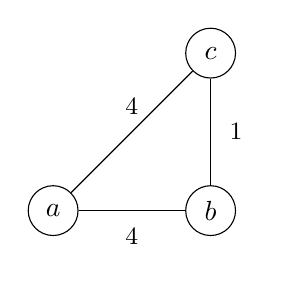
\begin{tikzpicture}[every node/.style={circle,draw,inner sep=2pt,minimum size=18pt},
                    lbl/.style={draw=none,fill=none,font=\small}]
  \node (a) at (0,0) {$a$};
  \node (b) at (2,0) {$b$};
  \node (c) at (2,2) {$c$};
  \draw (a)--(b) node[lbl,below,midway]{4};
  \draw (a)--(c) node[lbl,above,midway]{4};
  \draw (b)--(c) node[lbl,right,midway]{1};
\end{tikzpicture}
\end{center}

\textbf{Dijkstra from $a$:} $\mathrm{dist}[b]=4$ via $a$--$b$; $\mathrm{dist}[c]=4$ via $a$--$c$ (or $a$--$b$--$c$=5, so $a$--$c$ is used).
SPT $= \{a\text{-}b,\; a\text{-}c\}$, weight $= 8$.

\textbf{MST (Kruskal):} add $b$--$c$ (1), then $a$--$b$ (4).
MST $= \{b\text{-}c,\; a\text{-}b\}$, weight $= 5$.

The SPT includes edge $a$--$c$ (weight~4) which is not in the MST; the MST includes edge $b$--$c$ (weight~1) which is not in the SPT.  The SPT minimises \emph{path lengths from the source}, while the MST minimises \emph{total edge weight}; these are different objectives, so they generally produce different trees.

\newpage
\section*{Question 5: LCS Problem}

\subsection*{(a) What is memoization?}

Memoization is a technique in which the results of expensive function calls are stored (cached) the first time they are computed and then returned directly on subsequent calls with the same inputs, avoiding redundant recomputation.  It converts a recursive algorithm whose call tree has overlapping subproblems into one with polynomial time complexity.

\subsection*{(b) Subsequence vs.\ substring}

A \textbf{subsequence} of a string $S$ is any string formed by deleting zero or more characters from $S$ \emph{without changing the order} of the remaining characters.  The deleted characters need not be contiguous.

A \textbf{substring} is a \emph{contiguous} block of characters of $S$.

\textbf{Example.}  For $S = \texttt{ALGORITHM}$:
\begin{itemize}
  \item $\texttt{ALGO}$ is both a substring and a subsequence.
  \item $\texttt{AGRT}$ is a subsequence (positions 1,3,5,7) but \emph{not} a substring.
  \item $\texttt{LGOR}$ is \emph{neither} (order is violated).
\end{itemize}

\subsection*{(c) LCS of \texttt{ABFFSDERW} and \texttt{WFDFTRESAWE}}

Let $X = \texttt{ABFFSDERW}$ (length 9) and $Y = \texttt{WFDFTRESAWE}$ (length 11).

The DP recurrence is:
\[
dp[i][j] =
\begin{cases}
0 & \text{if } i=0 \text{ or } j=0 \\
dp[i-1][j-1]+1 & \text{if } X[i]=Y[j] \\
\max(dp[i-1][j],\, dp[i][j-1]) & \text{otherwise}
\end{cases}
\]

\begin{center}
\renewcommand{\arraystretch}{1.1}
\begin{tabular}{c|c|cccccccccccc}
& & \textbf{} & \textbf{W} & \textbf{F} & \textbf{D} & \textbf{F} & \textbf{T} & \textbf{R} & \textbf{E} & \textbf{S} & \textbf{A} & \textbf{W} & \textbf{E} \\ \hline
& \textbf{} & 0 & 0 & 0 & 0 & 0 & 0 & 0 & 0 & 0 & 0 & 0 & 0 \\
\textbf{A} & & 0 & 0 & 0 & 0 & 0 & 0 & 0 & 0 & 0 & 1 & 1 & 1 \\
\textbf{B} & & 0 & 0 & 0 & 0 & 0 & 0 & 0 & 0 & 0 & 1 & 1 & 1 \\
\textbf{F} & & 0 & 0 & 1 & 1 & 1 & 1 & 1 & 1 & 1 & 1 & 1 & 1 \\
\textbf{F} & & 0 & 0 & 1 & 1 & 2 & 2 & 2 & 2 & 2 & 2 & 2 & 2 \\
\textbf{S} & & 0 & 0 & 1 & 1 & 2 & 2 & 2 & 2 & 3 & 3 & 3 & 3 \\
\textbf{D} & & 0 & 0 & 1 & 2 & 2 & 2 & 2 & 2 & 3 & 3 & 3 & 3 \\
\textbf{E} & & 0 & 0 & 1 & 2 & 2 & 2 & 2 & 3 & 3 & 3 & 3 & 4 \\
\textbf{R} & & 0 & 0 & 1 & 2 & 2 & 2 & 3 & 3 & 3 & 3 & 3 & 4 \\
\textbf{W} & & 0 & 1 & 1 & 2 & 2 & 2 & 3 & 3 & 3 & 3 & 4 & 4 \\
\end{tabular}
\end{center}

The LCS length is $dp[9][11] = 4$.  Tracing back through the table:
$(9,11)\to(8,11)\to(7,11)\xrightarrow{E=E}(6,10)\to(5,10)\to(5,9)\to(5,8)\xrightarrow{S=S}(4,7)\to(4,6)\to(4,5)\to(4,4)\xrightarrow{F=F}(3,3)\to(3,2)\xrightarrow{F=F}(2,1)$.

Characters matched (in order): $F,F,S,E$.

\[
\boxed{\mathrm{LCS} = \texttt{FFSE}, \quad \text{length } 4}
\]

\bigskip
\noindent\textbf{References}\\
{[1]} T.\ H.\ Cormen \textit{et al.}, \textit{Introduction to Algorithms}, 3rd ed., MIT Press, 2009.\\
{[2]} J.\ Erickson, \textit{Algorithms}, 2019.

\end{document}
